\section{3-Class Classification}
In this section we discuss the multi-class method\footnotemark\footnotetext{Multi here refers to any non-binary number of classes}. Instead of only using sources which had AGN and PSR as their classification we added 108 sources in the 3FGL catalog which have a classification not falling under AGN or PSR. We gave them a classification of 'OTHER'. We ran our codes again, first to find the optimum parameters as was done in section 2. Figure \ref{fig:tree_multi} and \ref{fig:nets_multi} shows our results. Every method except the Neural Networks show the same behaviour as before and therefore we keep the same parameters for our final models. For Neural Networks the behaviour is also the same but the optimal parameter is found to be 600 epochs instead of 300. We keep the same number of neurons as before.


\begin{figure}[h]
\center
%\hspace*{-1cm}
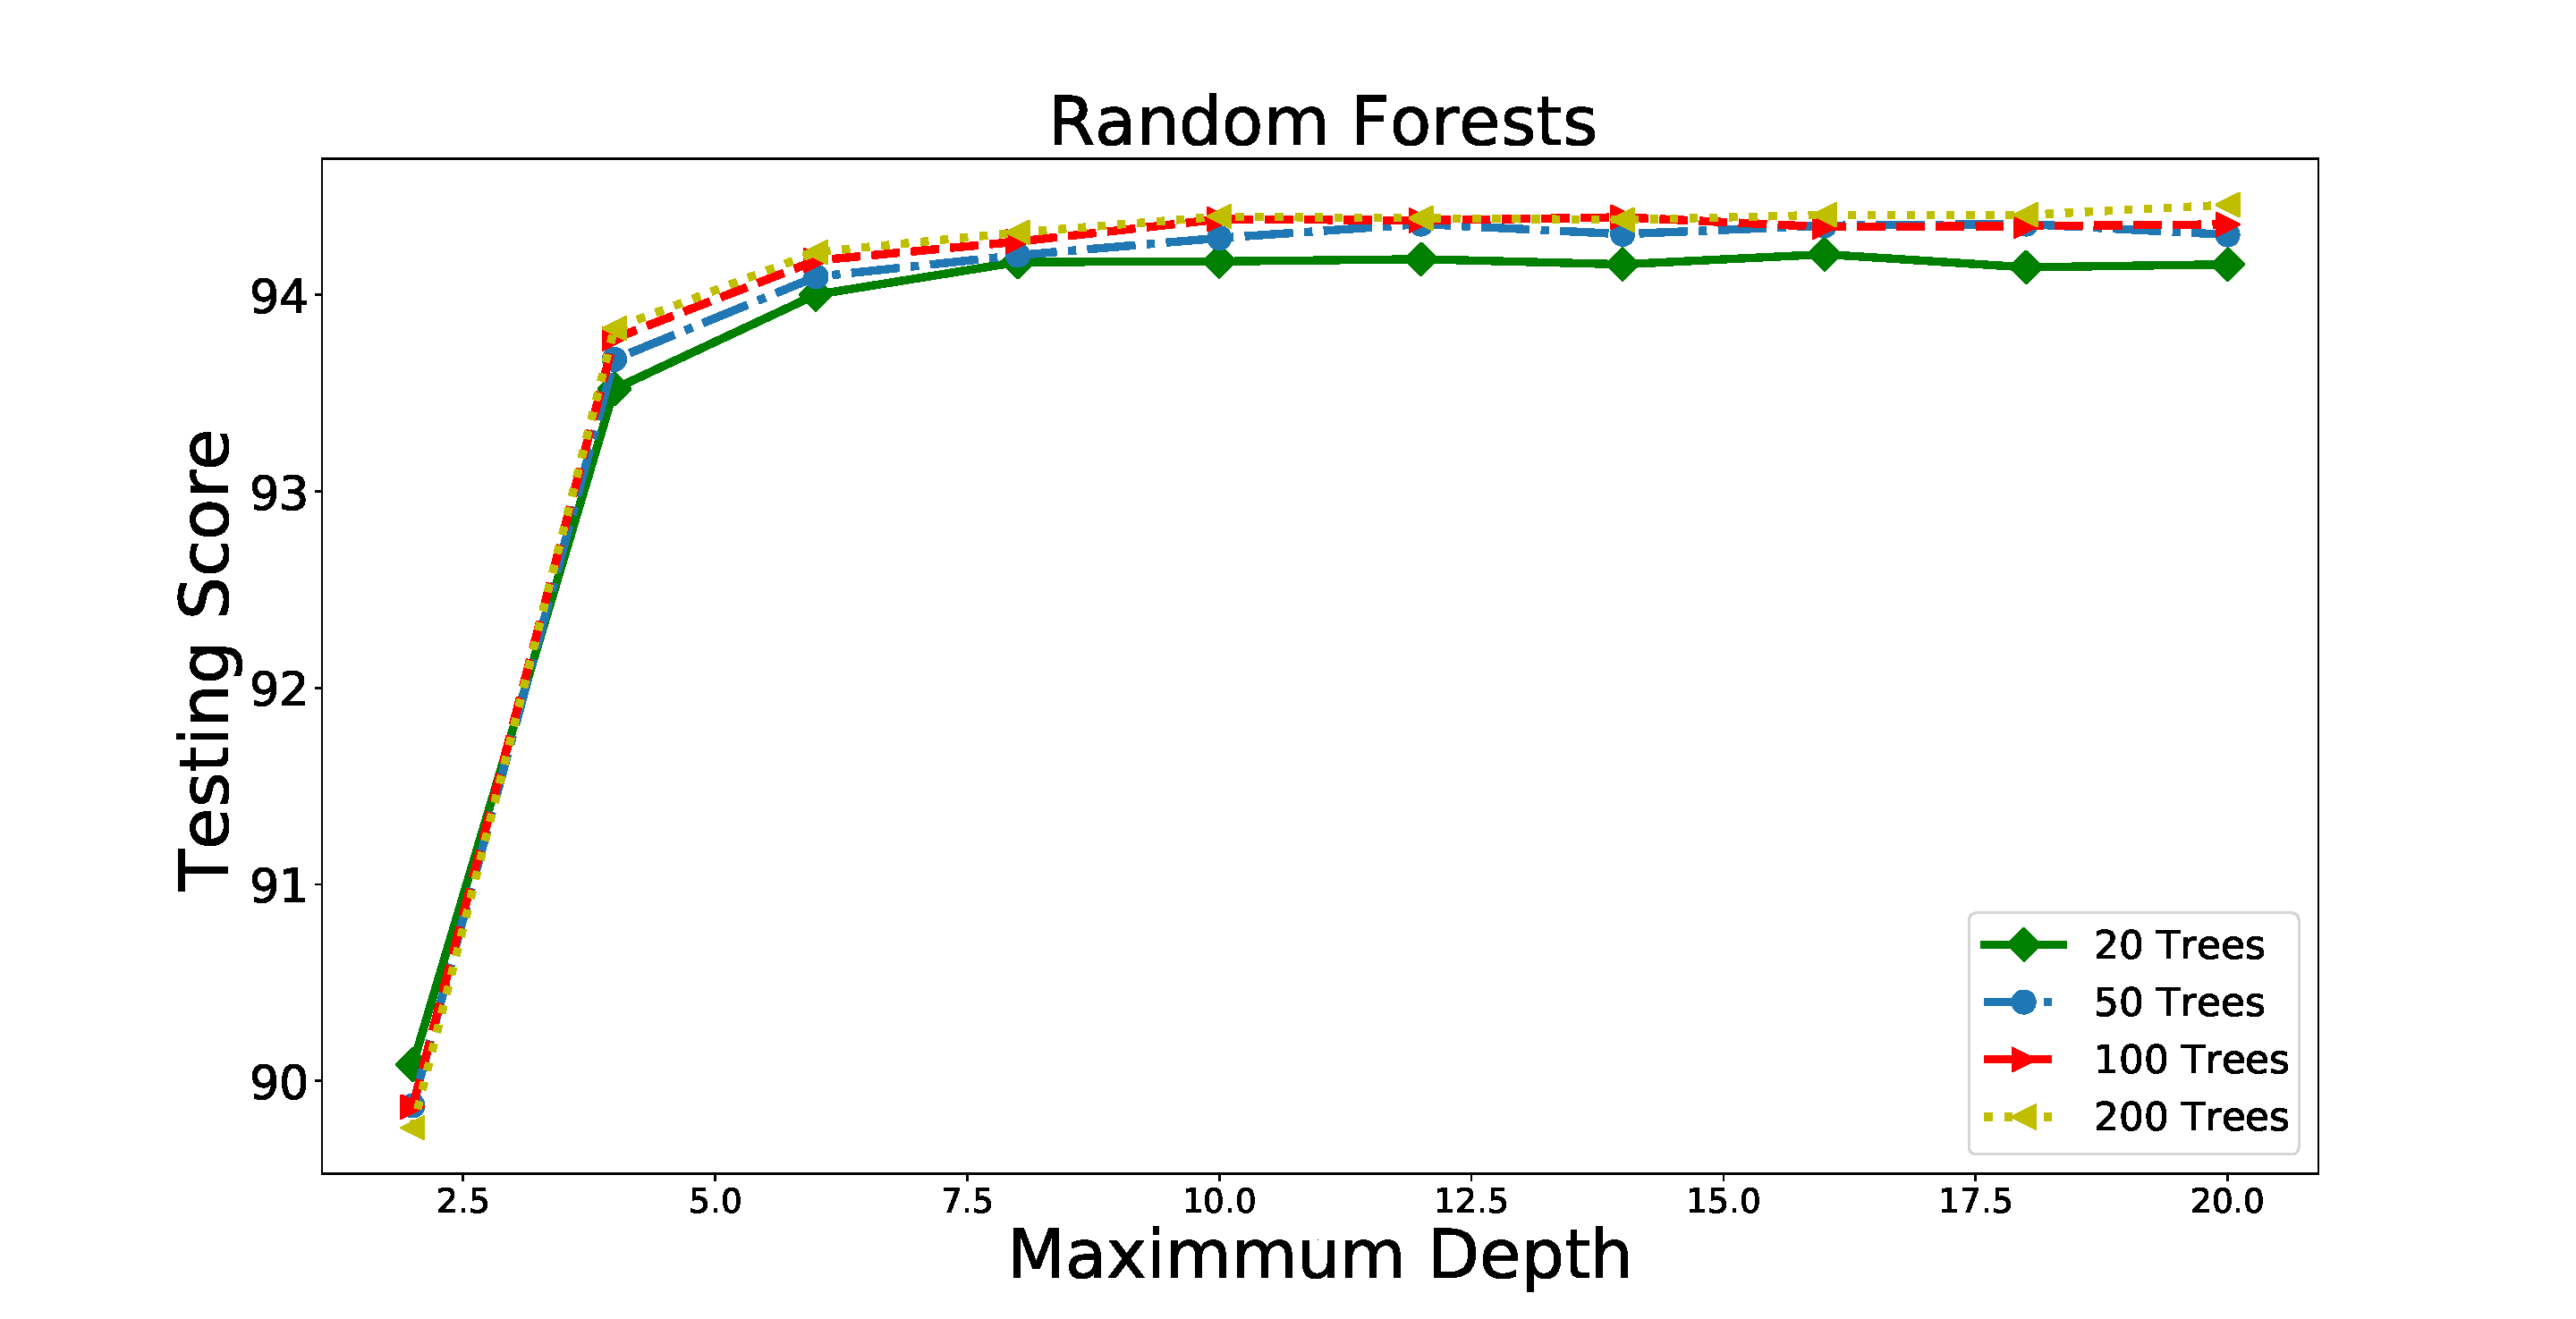
\includegraphics[width=0.5\textwidth]{plots/rf_train_multi.pdf}\\
%\hspace*{-1cm}
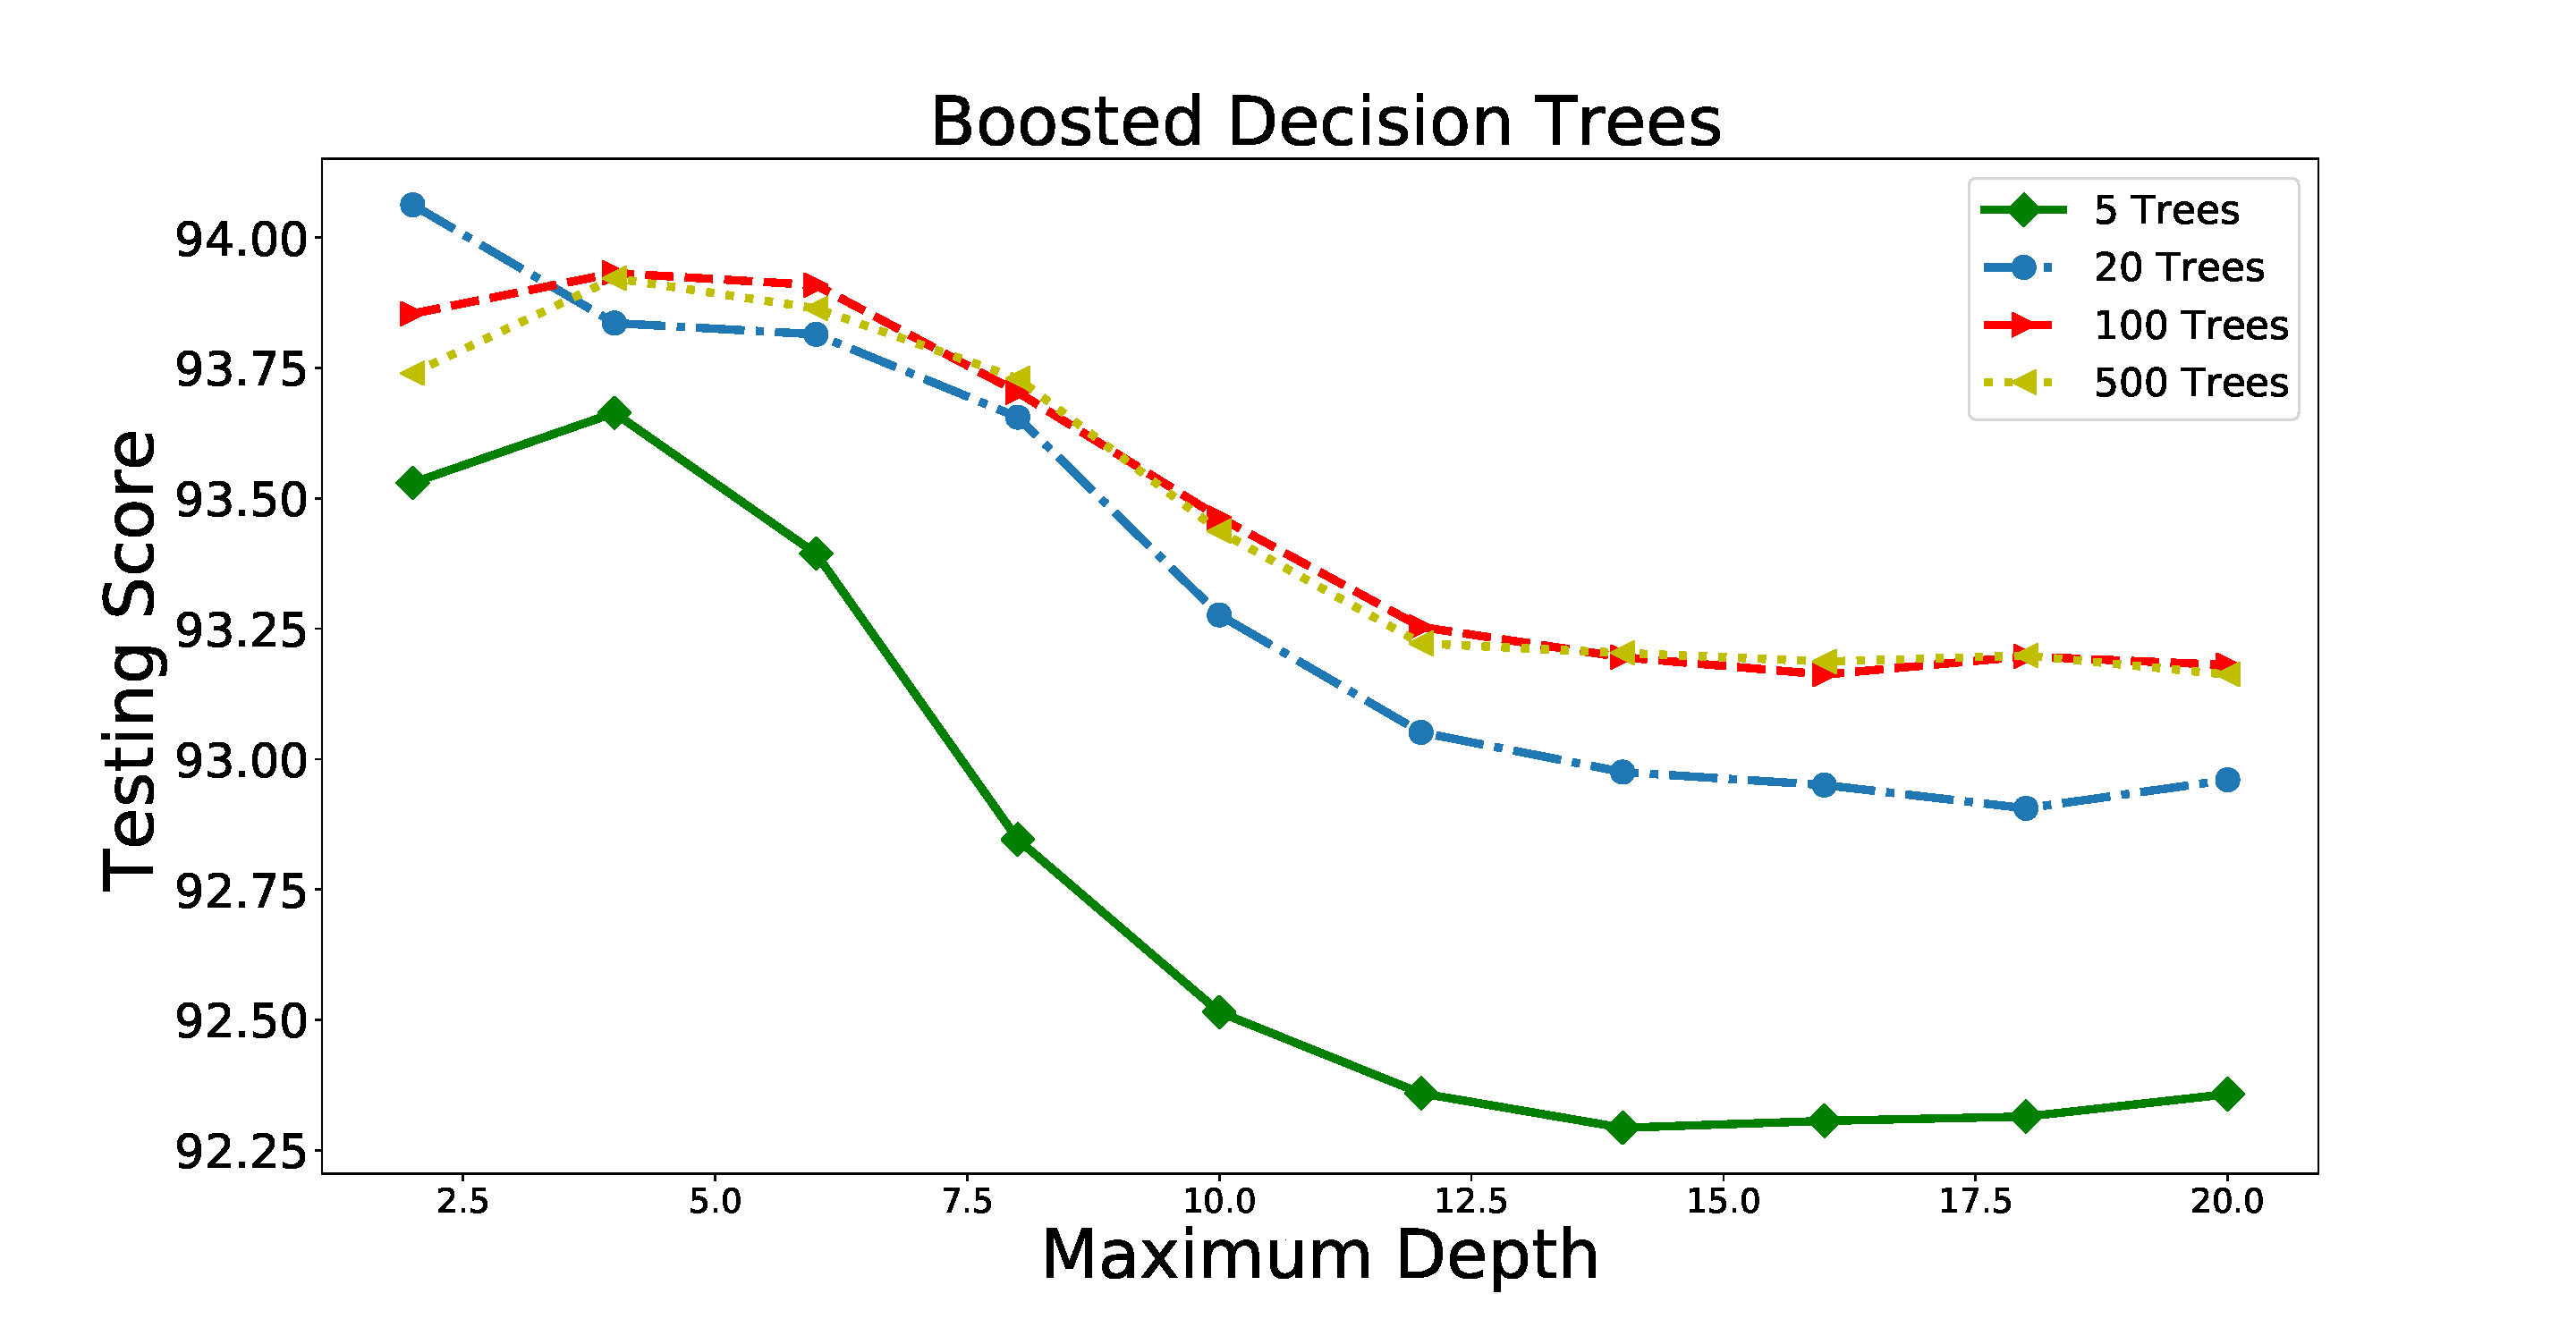
\includegraphics[width=0.5\textwidth]{plots/bdt_train_multi.pdf}
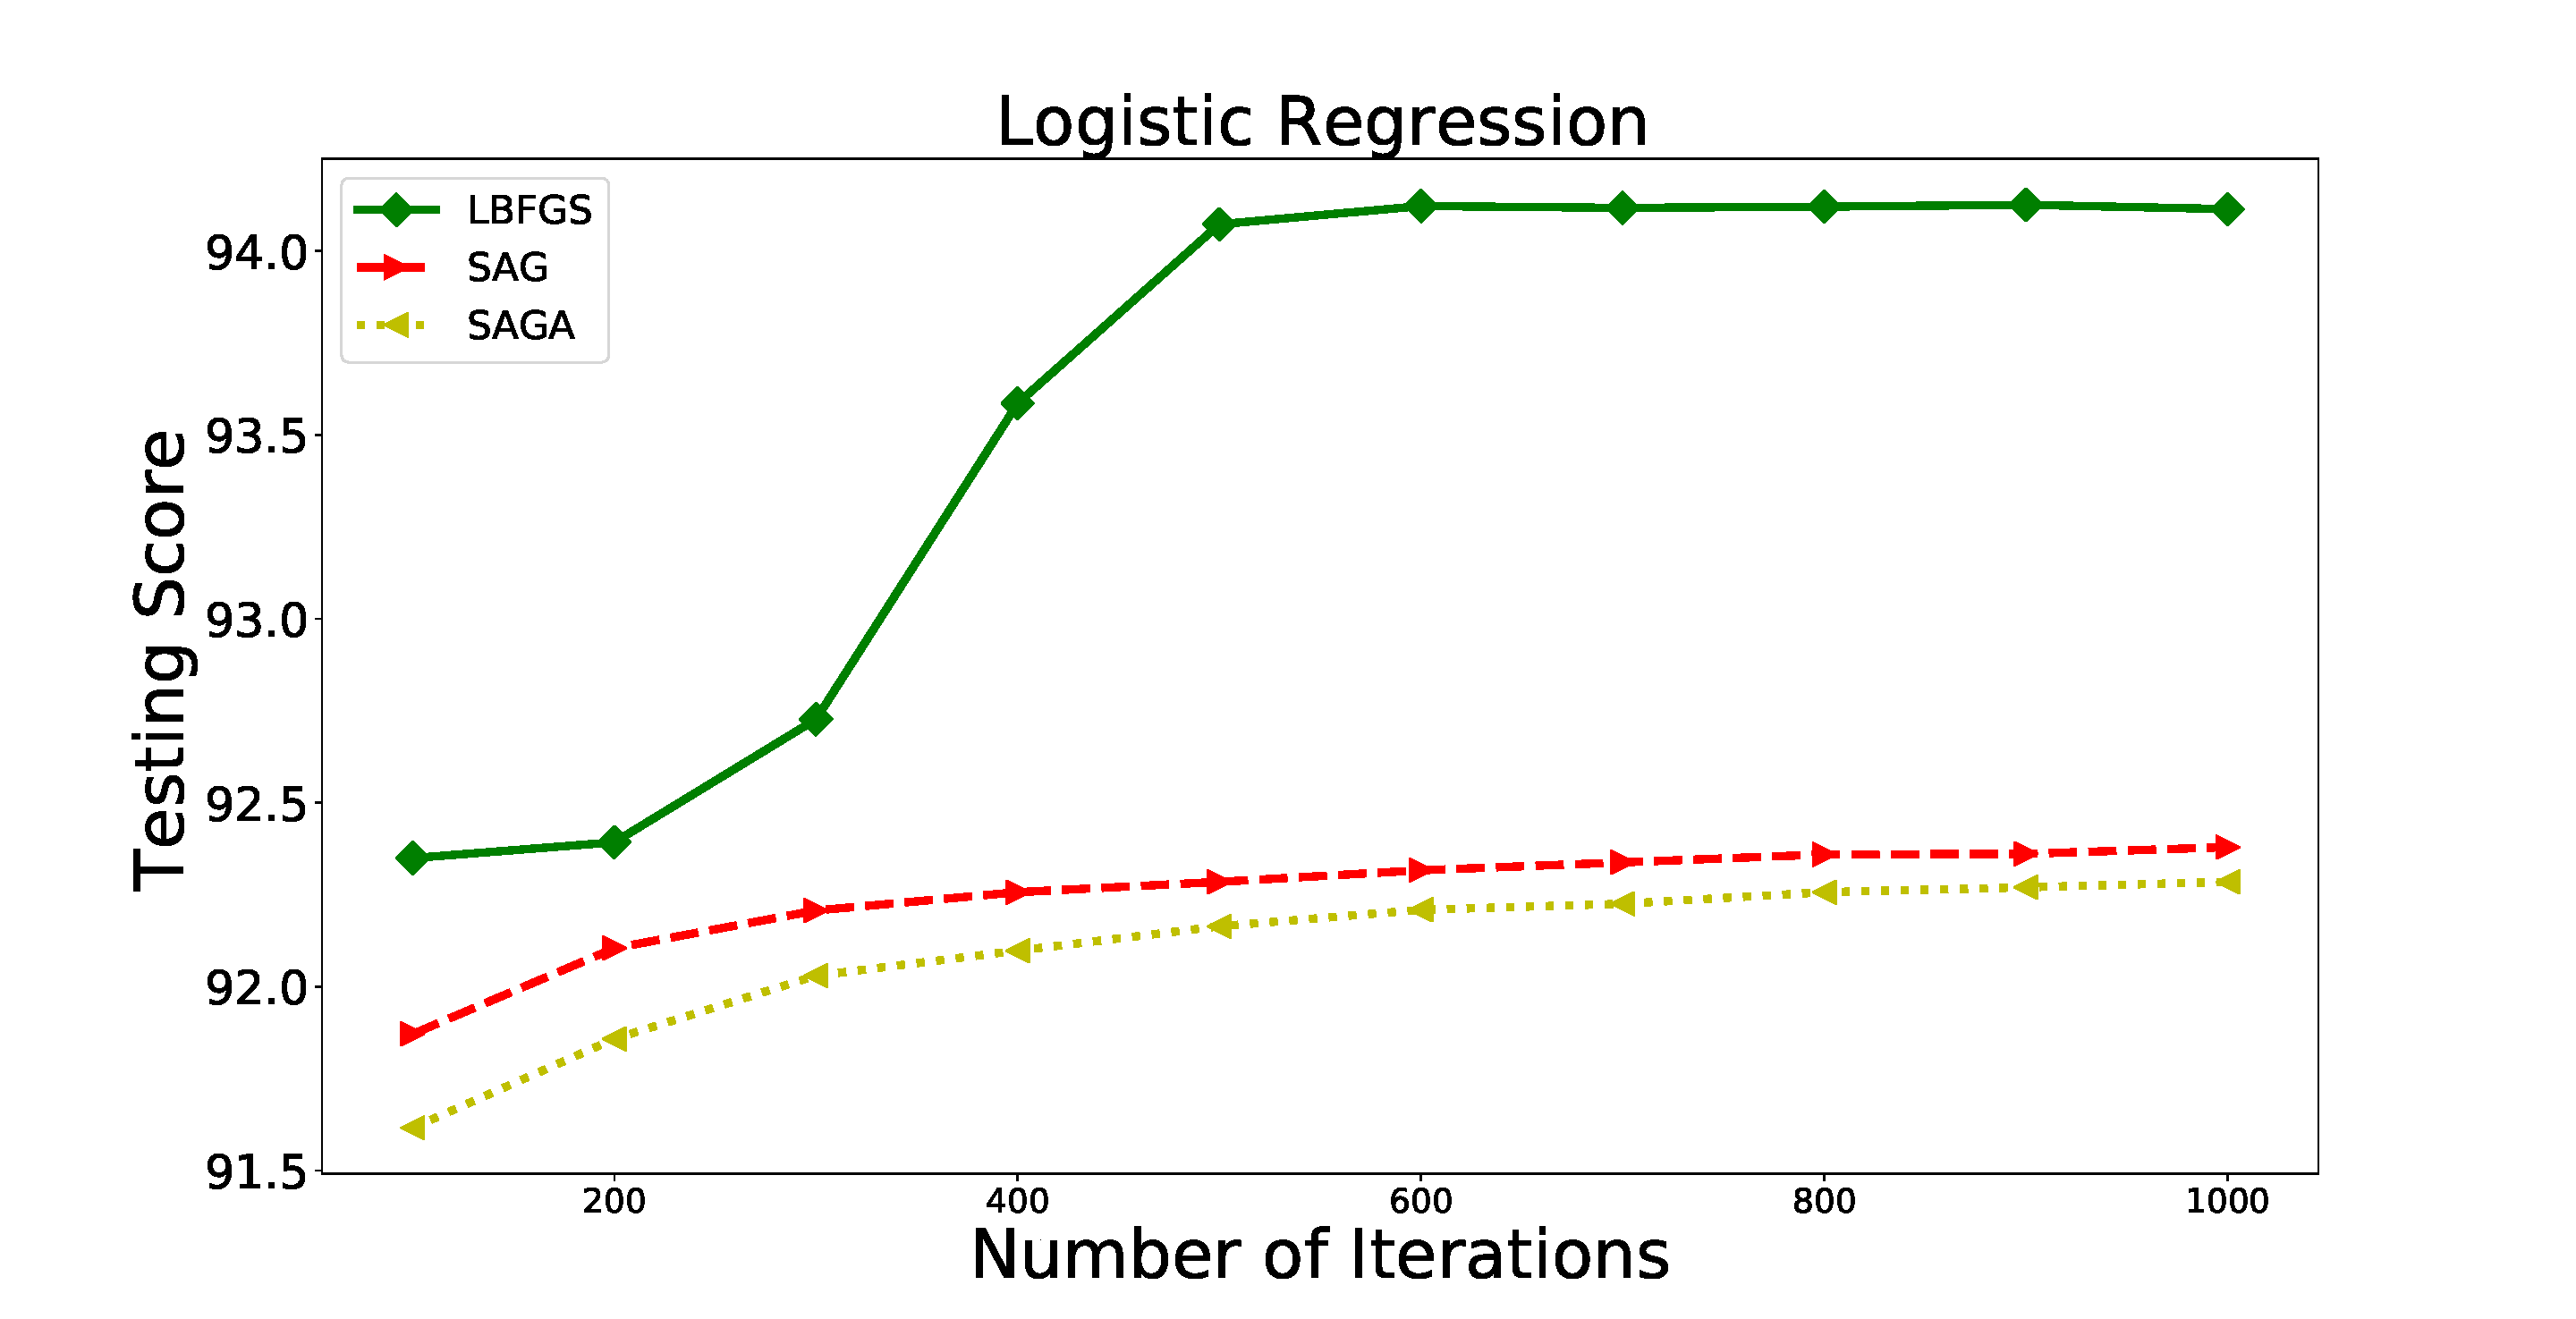
\includegraphics[width=0.5\textwidth]{plots/lr_train_multi.pdf}
\caption{Testing scores for classification methods of RF, BDT and LR.}
\label{fig:tree_multi}
\end{figure}
\begin{figure}[h]
\center
%\hspace*{-1cm}
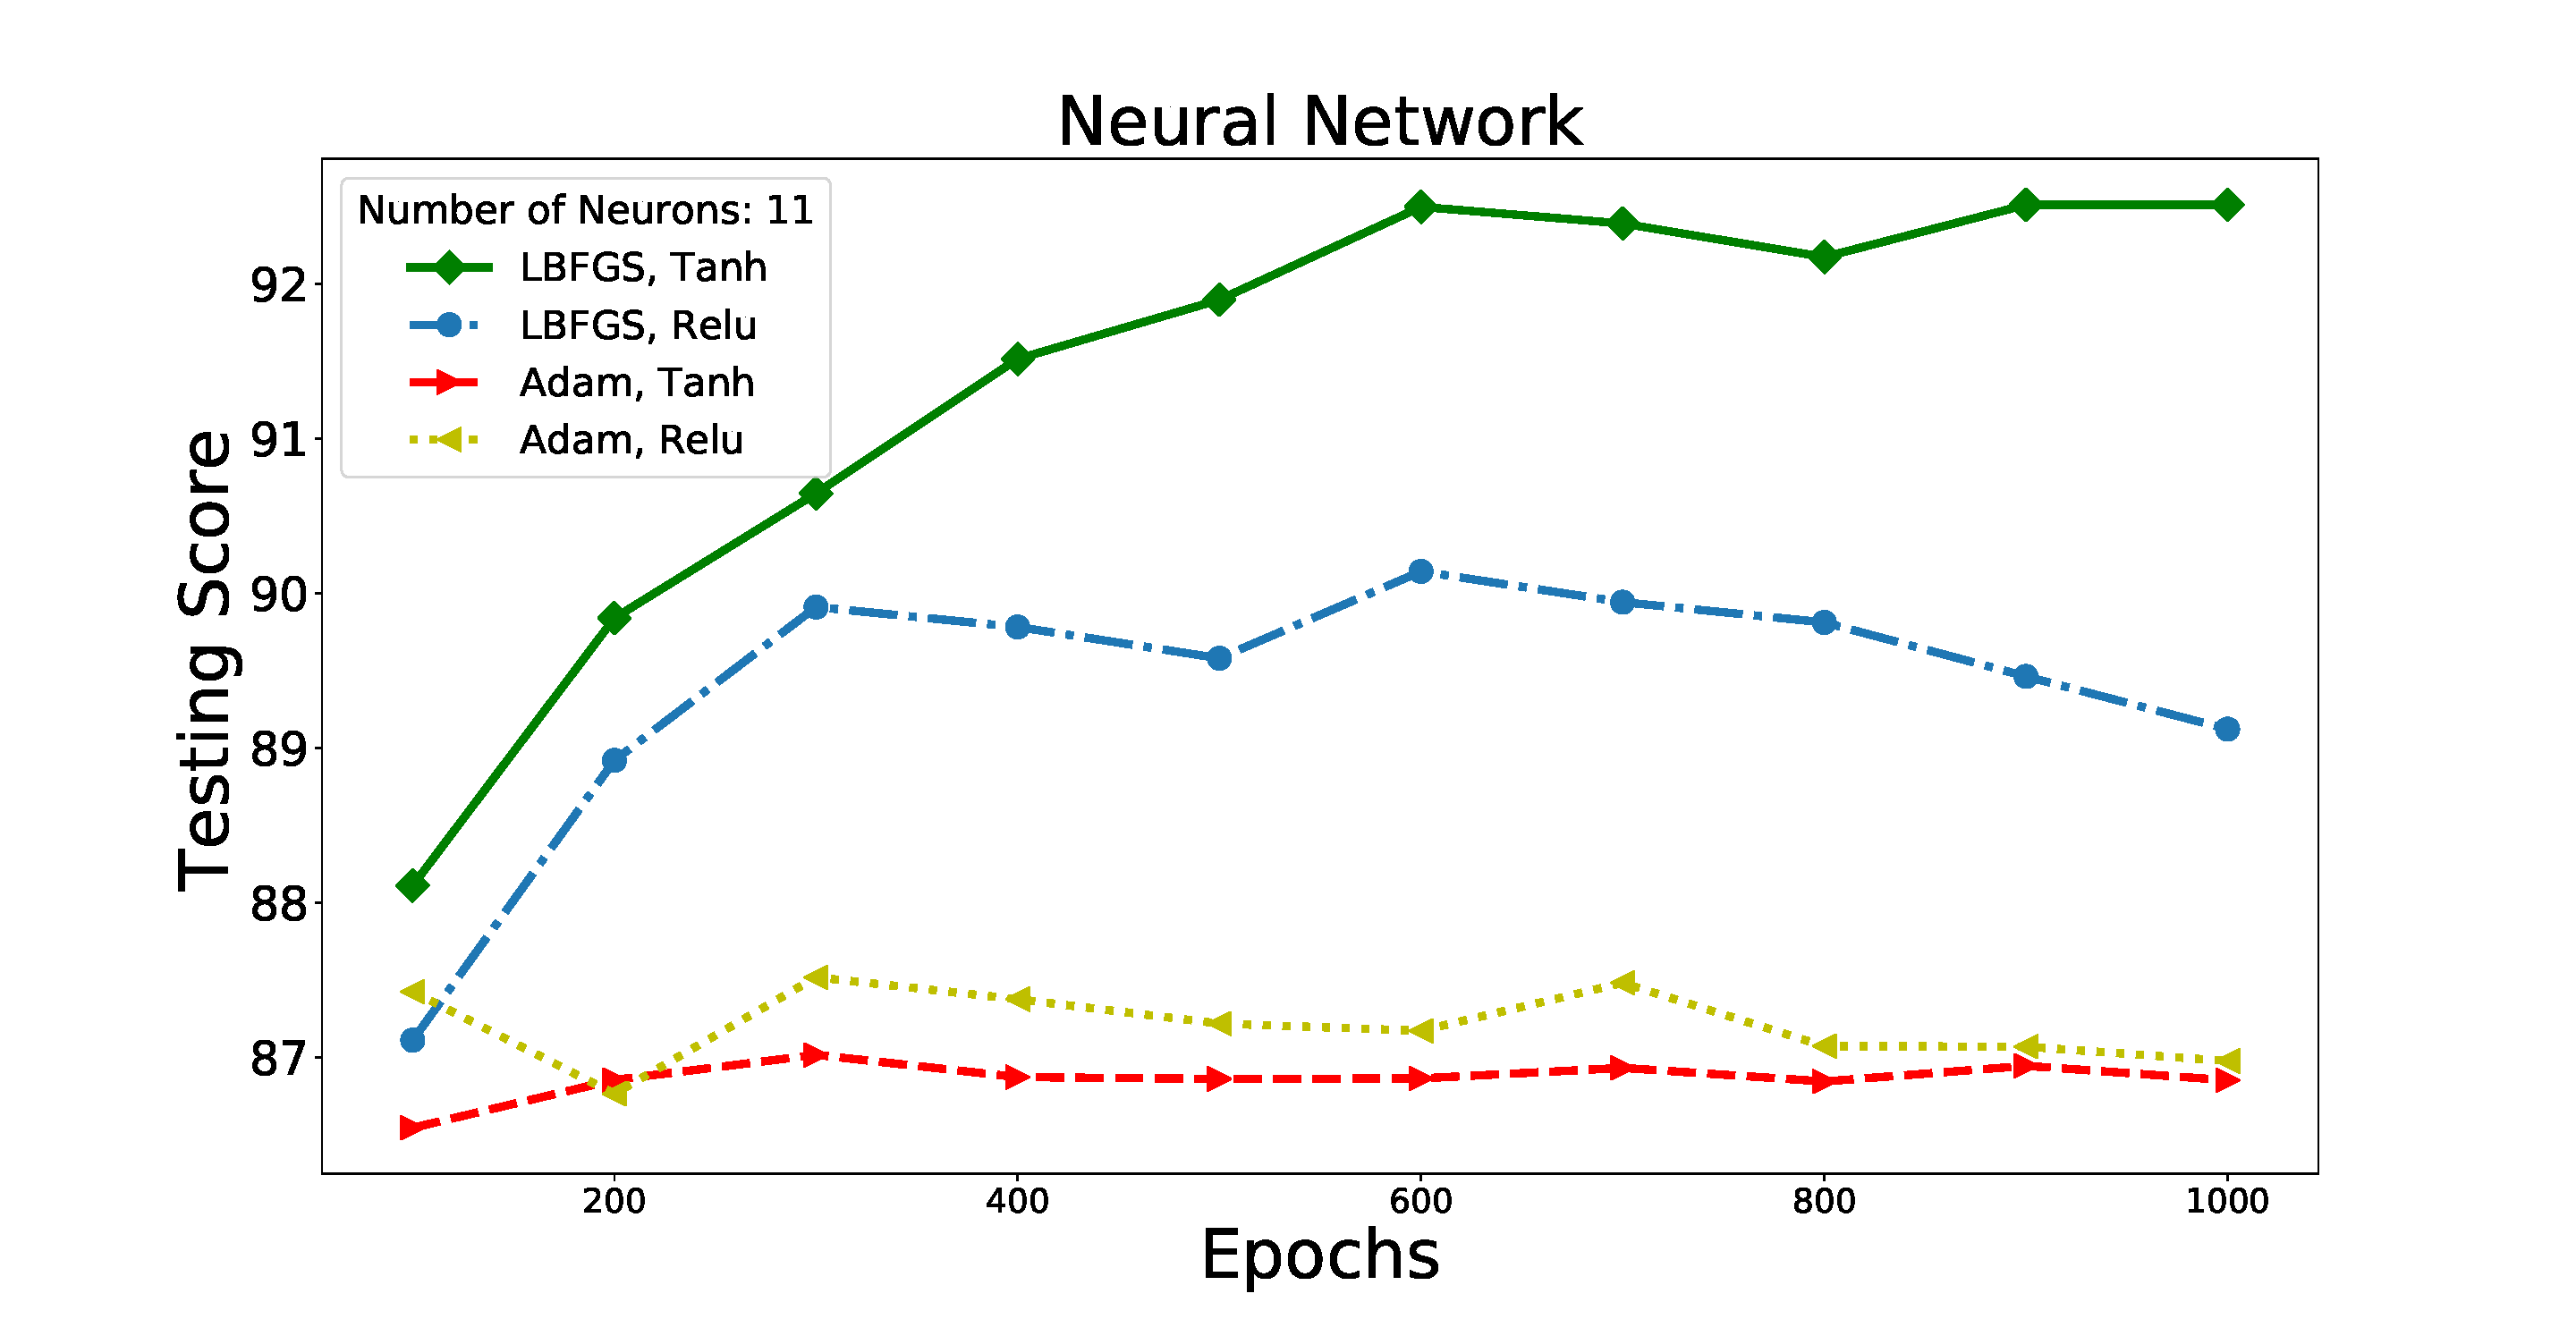
\includegraphics[width=0.5\textwidth]{plots/nn_epoch_train_multi.pdf}\\
%\hspace*{-1cm}
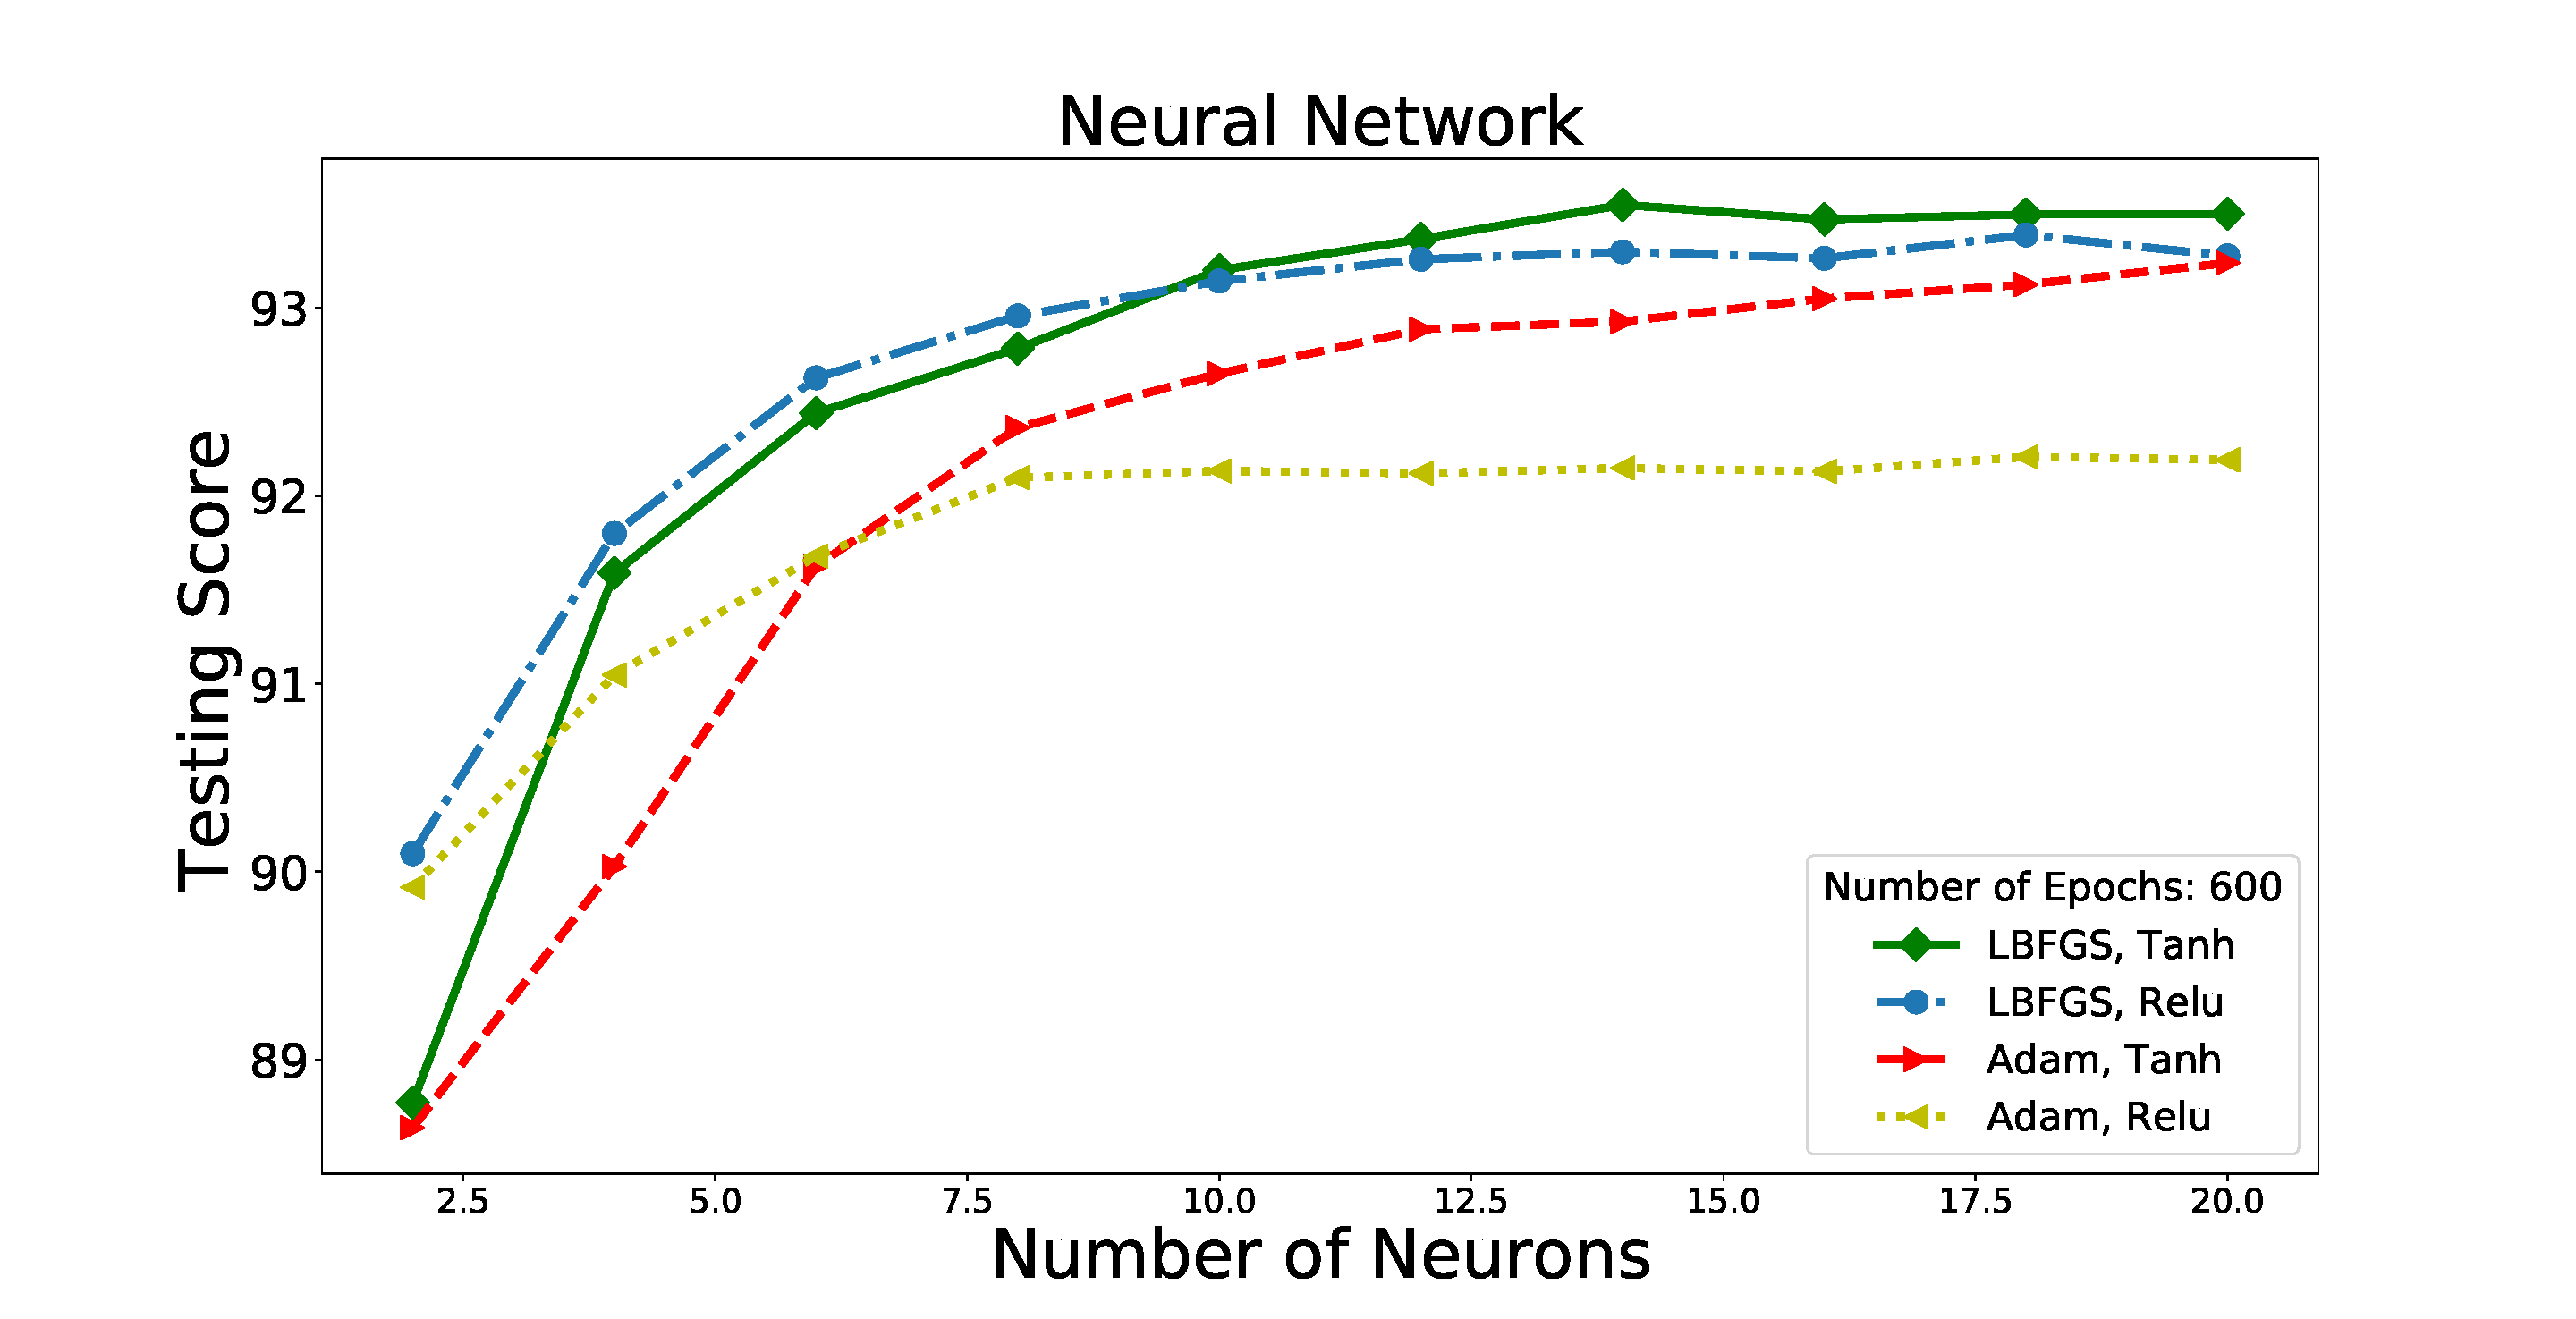
\includegraphics[width=0.5\textwidth]{plots/nn_neuron_train_multi.pdf}
\caption{Testing scores for classification methods of NN for a set number of Epochs and a set number of Neurons.}
\label{fig:nets_multi}
\end{figure}

The final accuracies of our chosen model for 1000 runs are given below in table \ref{tab:selected_algs_multi} for 3FGL and table \ref{tab:selected_algs_4fgl_multi} for 4FGL-DR2.
\begin{table}[!h]
\hspace{-0.2cm}
\resizebox{0.47\textwidth}{!}{
    \tiny
  \centering
    \renewcommand{\tabcolsep}{0.4mm}
\renewcommand{\arraystretch}{1.6}

%\hspace{-3mm}
    \begin{tabular}{|c|c|c|c|c|c|c|}
    \hline
    Algorithm&Parameters &  Testing&Std. Dev.& Comparison with 4FGL \\
    & & Accuracy & & Accuracy \\
    \hline
    RF & 50 trees, max depth 6  &93.90&0.84& 84.48  \\
    RF\_O &   &93.98&0.86& 85.35  \\
    \hline %\midrule   -> aakash do you mean this?
    BDT & 100 trees, max depth 2    &   93.66&0.84&83.67 \\
%    \hline %\midrule   -> aakash do you mean this?
%    BDT & 200 trees, max depth 2    &   95.8  \\
    BDT\_O &     &   93.34&0.85& 85.63 \\
    \hline
    NN & 600 epochs, 11 neurons, LBFGS & 92.22&1.40& 80.89\\
    NN\_O &&  79.74 &1.16& 69.66\\
    \hline
    LR & 200 iterations, LBFGS solver & 92.19&0.98& 80.68 \\
    LR\_O &  &75.55&2.03& 69.14 \\
    \hline
     
    \end{tabular}}
    \vspace{2mm}
    \caption{Testing accuracy of the 4 selected algorithms for classification of 3FGL sources and comparison with associations in the 4FGL-DR2 catalog. 
    ``\_O'' denotes training with oversampling.}
    \label{tab:selected_algs_multi}
\end{table}
\begin{table}[!h]
\hspace{-0.2cm}
\resizebox{0.47\textwidth}{!}{
    \tiny
  \centering
    \renewcommand{\tabcolsep}{0.4mm}
\renewcommand{\arraystretch}{1.6}
%\hspace{-3mm}
    \begin{tabular}{|c|c|c|c|c|c|}
    \hline
    Algorithm&Parameters &  Testing&Std. Dev.\\
    & & Accuracy &  \\
    \hline
    RF & 50 trees, max depth 6  &92.66&0.66  \\
    RF\_O &   &97.90&0.84 \\
    \hline %\midrule   -> aakash do you mean this?
    BDT & 100 trees, max depth 2    &   92.61&0.66 \\
%    \hline %\midrule   -> aakash do you mean this?
%    BDT & 200 trees, max depth 2    &   95.8  \\
    BDT\_O &     &   97.79&0.51 \\
    \hline
    NN & 600 epochs, 11 neurons, LBFGS & 91.62&0.78\\
    NN\_O &  & 94.31&5.13\\
    \hline
    LR & 200 iterations, LBFGS solver & 91.84&0.69 \\
    LR\_O &  &93.68&0.99\\
    \hline
     
    \end{tabular}}
    \vspace{2mm}
    \caption{Testing accuracy of the 4 selected algorithms for classification of 4FGL-DR2 sources. 
    ``\_O'' denotes training with oversampling.}
    \label{tab:selected_algs_4fgl_multi}
\end{table}